\subsection{Project description}
The project is part of the course TDT4290 Customer Driven Project. This course
is mandatory for all computer science majors, and its goal is to give the
students experience with customer relations, project management and group
dynamics in a real project.

The project itself is about developing a cross-compiling application for mobile
platforms. We are to deliver a study of different frameworks, the project
process, and an evaluation of the process and framework used. The application
will aid observers in the field, and seeks to replace the old notebook-way of
gathering species observations in the field. The project is sponsored by
Artsdatabanken.

In this section, we will look at the project, the people involved, and the
limitations of the project.

\subsubsection{The customer}
Our customer is Artsdatabanken. Artsdatabanken is a company in the
Norwegian Biodiversity Information Center (NBIC) body that provides the
public with information on Norwegian species and ecosystems.
Artsdatabanken claims to have approximately 6 million species of plants,
insects, birds, large predators. Of these 6 million, 85\% are birds.
Artsdatabanken keeps a series of database resources such as Red List,
Alien Species, Species name and Habitat databases together with Species
Map and Species Observations. Artsdatabanken depends on these projects
and databases to fully conduct its operations and
responsibilities.\cite{artsdatabanken:about}

\subsubsection{People involved in the project}
The student group consists of seven fourth year students partaking the Computer
Science program at the Norwegian University of Science and Technology. Two of
these students are enrolled in the International student exhange program for
Computer Science. These are in alphabetical order: Anders Søbstad Rye, Andreas
Berg Skomedal, Dag-Inge Aas, Muhsin Günaydin, Nikola Djoric, Stian Liknes and
Yonathan Redda. The student group is advised by PhD Candidate, Muhammad Asif, at
IDI.

The customers representatives are Askild Olsen and Helge Sandmark. Askild Olsen
will function as the product owner, and has the final word when decisions are
made about the project. They are employees of Artsdatabanken, where they are
responsible for development and maintenance of existing systems. 

\subsubsection{Project drivers}
Artsdatabanken has a very skilled user base. Some of the users have for a long
time requested a mobile application for gathering observation data in the
field. This application would replace the old notebook method of gathering
information, automate collection of some data such as GPS coordinates, and
decrease the complexity involved in making observations of species, so that
beginners would have an easier time learning the process. In addition,
Artsdatabanken wants the application to help increase the number of
observations by increasing the number of users and significantly lessen the
complexity involved in registering observations.

\subsubsection{Problem domain}
In the current situation, an observer has to make the observation, write down
the number of individuals in each species and alternatively take a picture. After this is done,
the observer must go home, post everything to an online form and
alternatively upload pictures separately. Because of the complexity and the
lack of automation involved in this process, the smaller observations are often
overlooked, and doesn't get registered. Artsdatabanken wants as many
observations done as possible.

In addition, considering that Artsdatabanken is a public institution brings
additional demands to the project. Artsdatabanken needs to support as many
mobile devices as possible. This means that the application must work on
a variety of devices with different operating systems and screen sizes.

\subsubsection{Proposed solution}
Our proposed solution involves using a cross-compiling mobile application
framework, named Phonegap, that can deploy the same code on multiple platforms.
This will enable us to use the same codebase, but deploy on six different
platforms. The application itself will automate a lot of the data collection
involved with making observations, and exports the data to a computer-readable
format suitable for parsing by Artsdatabankens systems. This solution will
lower the barrier for making and registering observations, enabling more users
to partake.

\subsubsection{Project objective}
The student group are expected to deliver a common mobile application codebase
that can be deployed on many different platforms in addition to a working
application demo that can export observations ready for parsing by the server.
The server-side APIs will be provided by Artsdatabanken. In addition, the
student group will deliver all research made into the problem domain to the
customer, including research into cross-platform frameworks and deployment.

\subsubsection{Available resources}
Artsdatabanken will provide user testing of the application. They will also be giving a short taxonomy training to a few selected students and hold a field study, giving the
students the opportunity to learn about observations and species.

The students will supply testing hardware for the Android platform, and the customer is expected to provide an i family device for iOS application testing. This gives the students the opportunity to test
the application on the two most popular platforms in various screen sizes.

\subsubsection{Limitations}
The project is scheduled to last from the 30th of August to the 24th of
November. The budgeted working hours per group member is 350 hours, making the
total working hours available to 2450  person hours. This is equal to over one
year worth of person hours. Time could possibly be one of our limitations in the project.

As the students have no testing hardware for Symbian, Bada, BlackBerry or
Windows Phone, the applications developed for these platforms will not be
tested on a real device prior to launch. The students also lack hardware
necessary for efficient testing of the application on Apple's iOS platform, having to rely only on sporadic
access to the hardware. OS Hardware being the best testing platform, the lack of them will certainly have its limits on our testing capability in this project.
<<<<<<< HEAD
=======

\subsubsection{Similar products}
We explored similar products for inspiration and in the hope of finding
functionality possibilities that can easily be integrated in our product, but
not necessarily dictated by our customer. Besides, the team thought it could
learn something which is going to be new and some which were already tried.
General opinions are that commercial-off-the-shelf software are thought to be
straight forward, time and cost saving even thought it might bring its own
version of problems\cite{similarproduct:introdn}. Having said that, we
summarized what were closer to the system we are developing below.
\paragraph{Project Noah - Networked Organisms and Habitats}

Project Noah is a mobile application that helps nature lovers discover local
wildlife and aspiring citizen scientists contribute to current research
projects. Noah stands for networked organisms and habitats. It is a tool people
can use to document and learn about their  natural surroundings and as a
technology platform research groups can  use to harness the power of citizen
scientists everywhere. And it documents species sighting with date, category,
habitat, picture and comments\cite{similarproduct:noah}. 

\begin{figure}[htb]
    \centering
    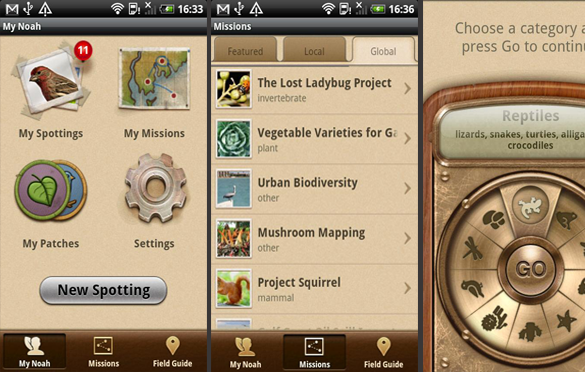
\includegraphics[width=0.8\textwidth]{introduction/project_description/noah.png}
    \caption{Projet Noah app}
    \label{fig:Noahapp}
\end{figure}

\paragraph{US Birding Checklist}
This is a bird watching tool set which records species sex, age location and
pictures\cite{similarproduct:usbird}.

It uses an online database system called eBirds\cite{similarproduct:ebird},
which is launched and run by Cornell Lab of Ornithology and National Audubon
Society. It also show the distribution of birds on a map. 

\begin{figure}[htb]
    \centering
    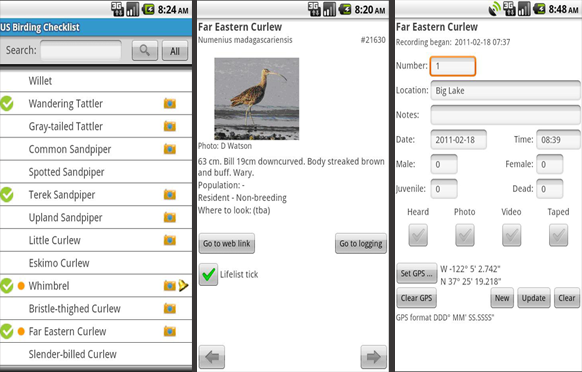
\includegraphics[width=0.8\textwidth]{introduction/project_description/usbirdingchecklist.png}
    \caption{US Bird Checklist app}
    \label{fig:usbirdapp}
\end{figure}

\paragraph{Audubon Guide}
Audubon is a portable dictionary like content provision on mobile phones. It
downloads a wealth of information about mammals, birds, butterflies and more on
the mobile phone and its focus is for viewing and providing information about
species\cite{similarproduct:audubon}. Audubon has a variety of version such as
Audubon Wildflowers, Audubon Butterflies, Audubon Mammals.

\begin{figure}[htb]
    \centering
    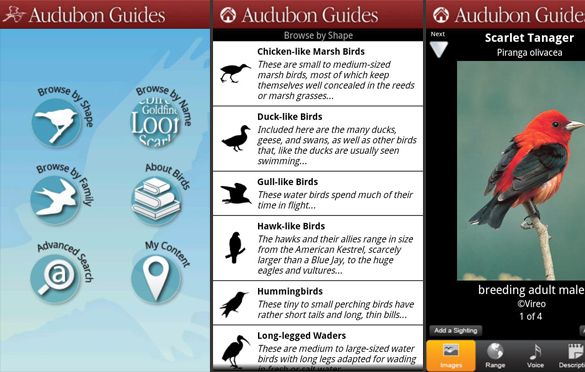
\includegraphics[width=0.8\textwidth]{introduction/project_description/audubonguide.png}
    \caption{Audubon species guide app}
    \label{fig:audubonapp}
\end{figure}

But we found none of the application fit for the requirements from
Artsdatabanken. Artsdatabanken runs its own data source and whatever COTS
(Commercial off-the-shelf) the team considers should enable Artsdatabaken to
access its data source. Artsdatabanken requirements recommend a strict inclusion
of requirements such as inclusion of location, pictures, number of species,
activity which are handled in a different ways in the applications described
above. The applications are also not free and  can be customized to our customer
needs, a lot more reason to resort to development.
>>>>>>> 0f2360b98b1050ada14d1650f7c4377418a2a5e0
